\section{\spork{} Design}
\label{sec:design}

\begin{tcolorbox}[
  colback=blue!3!white,
  colframe=blue!45!black,
  boxrule=0.45pt,
  arc=1.5pt,
  left=4pt,
  right=4pt,
  top=3pt,
  bottom=3pt
]
\textbf{Systems question.}
How can we overlap tool execution with main generation at minimal added overhead,
while keeping the agent lossless with respect to its serial execution?
\end{tcolorbox}

\noindent \spork{} answers with three mechanisms: \textbf{Design~1 (D1)},
\textbf{Design~2 (D2)}, and \textbf{Design~3 (D3)}, each grounded in one insight
from \S\ref{sec:selfspec} and targeting a specific parameter of the cost model
(EQ1, \S\ref{sec:eq1}).

At each agent turn, \spork{} runs the following pipeline (Figure~\ref{fig:method_overview}):
\begin{enumerate}
\item Dispatch the main generation as a streaming chat-completion request.
\item After the first streaming token, launch a fork thread that issues a raw
      completion request with a forced tool-call prefix.
\item The fork thread monitors its generation logprobs (D2); once confidence reaches a
      threshold $\theta$ (the confidence gate, \S\ref{sec:d2}), dispatch speculative
      tool execution.
\item When the main stream reaches its tool call, compare it against the committed
      probe under the gate criterion. On match: use the pre-computed result.
      On mismatch: fall back to serial tool execution. In the engine configuration,
      D3 has meanwhile served the probe's tool-call body to the main stream as
      speculative-decoding draft tokens, so the main decode re-emits only the tokens
      after the first mismatch rather than the whole call.
\end{enumerate}

The D1/D2 controller is a Python application-layer component that uses standard serving
APIs and collects no training data.
D3 additionally integrates with vLLM's speculative-decoding proposer path to inject
verified probe tokens as drafts; we describe this as a prototype integration rather than
a generic no-engine-modification claim.

\begin{figure*}[!t]
  \centering
  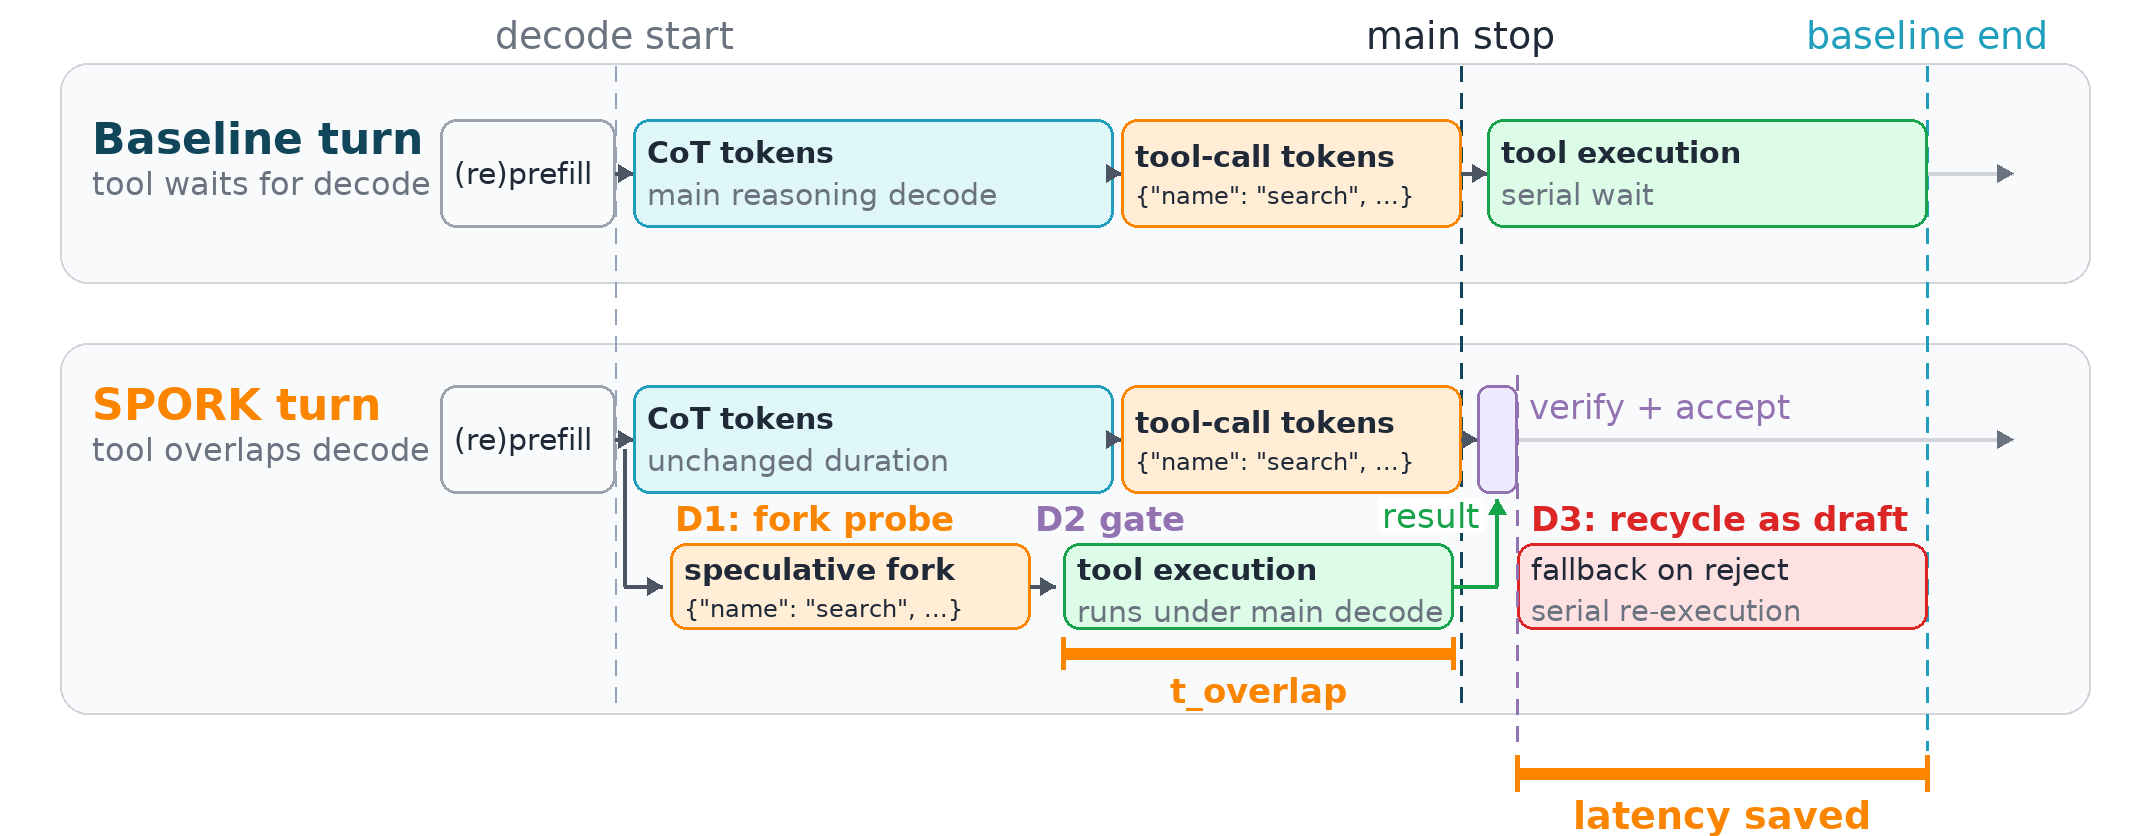
\includegraphics[width=\textwidth]{figures/fig2_method_overview_v2.png}
  \caption{\textbf{\spork{} method overview.} \textit{Top:} the baseline turn is strictly
  serial: (re)prefill, CoT decode, tool-call decode, then a stall while the tool
  executes. \textit{Bottom:} \spork{} forks the KV cache after the main's first token and
  launches a forced tool-call probe (\textbf{D1}); once the probe's logprob confidence
  clears the gate (\textbf{D2}), the predicted tool executes during the remaining decode,
  producing the overlap $t_{\mathrm{overlap}}$. A strict match at main-stream completion
  accepts the pre-computed result; on mismatch the turn falls back to serial execution and
  \textbf{D3} recycles the rejected probe's tokens as a speculative-decoding draft.}
  \label{fig:method_overview}
\end{figure*}

\parabf{EQ1 parameter mapping.}
Each mechanism targets a different term in the cost model
(Table~\ref{tab:design_rationale}; Eq.~\ref{eq:eq1}, \S\ref{sec:eq1}):
D1 follows Insight~1 and \emph{minimizes the overhead term} $\Toh$: by reusing the
main's prefix KV cache, the probe's cost collapses from 1.6\,s to 0.35\,s, and its
dispatch at the first streaming token opens the overlap window.
D2 follows Insight~2 and \emph{maximizes the expected overlap} $\alpha\cdot\toverlap$:
gating dispatch on the probe's own logprob confidence, it commits at the earliest probe
confident enough to act on, trading a slightly smaller window for much higher
acceptance.
D3 follows Insight~3 and lowers $\Tbasestar$ on misses by recycling the probe's verified
prefix as draft tokens, so the main stream re-decodes only the suffix after the first
mismatch.
Together, all three push the operating point toward the $\alpha\cdot\toverlap \geq \Toh$
break-even condition from both sides.

\begin{table}[tbp]
\caption{\textbf{Design rationale.} Each mechanism is tied to one insight and one
EQ1 term.}
\label{tab:design_rationale}
\centering
\small
\begin{tabular}{@{}lll@{}}
\toprule
Design & Insight & EQ1 effect \\
\midrule
\textbf{D1} & Insight~1 & minimizes $\Toh$ \\
\textbf{D2} & Insight~2 & maximizes $\alpha\cdot\toverlap$ \\
\textbf{D3} & Insight~3 & lowers $\Tbasestar$ (miss re-decode) \\
\bottomrule
\end{tabular}
\end{table}

\spork{} composes the three mechanisms. D1+D2 form the training-free controller, and D3 adds
engine-side partial-token recovery. The ablation in \S\ref{sec:ablation} measures each
mechanism's contribution.
The controller is stateless across turns except for the shared prefix cache inside the
serving engine: each agent turn forks independently, and the gate always compares against
the main stream's final tool call before any result is committed to the conversation history.

\subsection{D1: Prefix-Cache Fork for Near-Zero Probe Overhead}
\label{sec:d1}

\parabf{Mechanism.}
The probe is not free, since it must generate a tool call of its own; its overhead
decomposes into a decoding cost and a prefilling cost.
The decoding cost is small.
The fork decodes only the tool-call body (typically $\leq 50$ tokens, stopping at the
tool-call close), $10\text{--}50\times$ shorter than the main's CoT, about 0.3\,s on
Qwen3-32B at 15K context.
The prefilling cost is the heavy part: the fork shares the full prompt prefix
(system + user + history) with the main request, and re-prefilling it costs
$\sim$1.3\,s at the same context; worse, we measure that dispatching the fork
simultaneously with the main request causes 2.5$\times$ prefill contention.
Modern LLM serving systems such as vLLM~\citep{kwon_efficient_2023} and
SGLang~\citep{zheng_sglang_2024} cache prefix KV states; D1 therefore
dispatches the fork \emph{after} the main's first streaming token.
Because the main request has by then populated the prefix cache, the fork's prefill is
a cache hit at near-zero cost ($\sim$0.05\,s), and the staggered dispatch reduces
prefill interference to $<1\%$.
With D1, probe overhead collapses from 1.6\,s (1.3\,s prefill + 0.3\,s decode) to
0.35\,s (0.05\,s cache-hit prefill + 0.3\,s decode).
Figure~\ref{fig:d1_overhead} shows the resulting end-to-end effect: the fork's measured
TPOT overhead on the main stream is within intrinsic batching noise.

\begin{figure}[t]
  \centering
  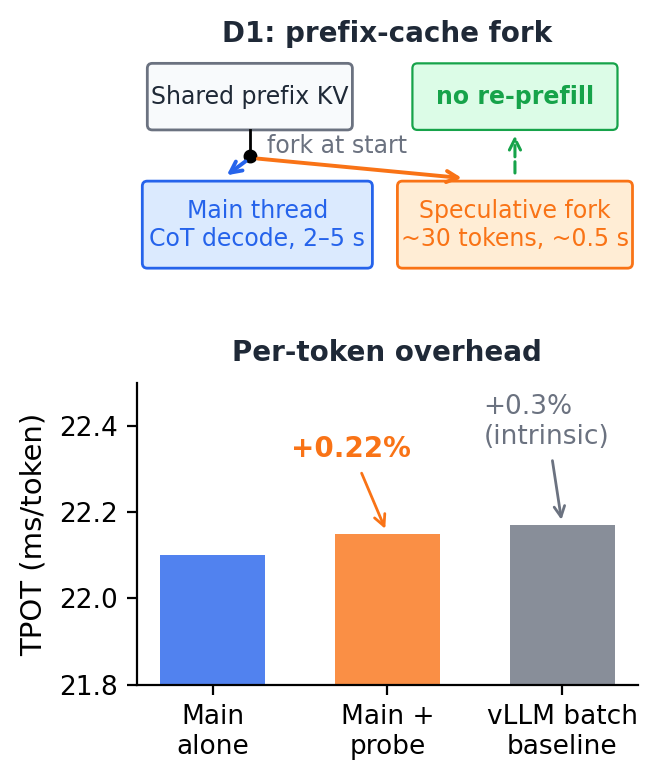
\includegraphics[width=0.95\columnwidth]{figures/fig_d1_overhead.png}
  \caption{\textbf{D1 reuses the prefix KV cache to keep probe overhead small.}
  Probe TPOT overhead (+0.22\%) is within intrinsic batching noise (+0.3\%).}
  \label{fig:d1_overhead}
\end{figure}

\subsection{D2: Adaptive Confidence Gate}
\label{sec:d2}

\parabf{Motivation.}
Without gating, D1 dispatches speculative tool execution on \emph{every} fork, regardless
of whether the probe is likely correct.
Each wasted dispatch consumes network/compute resources and, on side-effecting tools, must
be rolled back.
Insight~2 (\S\ref{sec:selfspec}) shows that probe accuracy improves dramatically with
context: argument accuracy rises from 7.6\% at 0\% CoT to 97.5\% at 100\% CoT
(Figure~\ref{fig:cot_curve}).
D2 exploits this by \emph{not committing} until the fork's own token-level confidence
signals that the generated tool call is likely correct, enabling the system to filter
out low-quality probes before they trigger wasted work.

\parabf{Confidence metric.}
The fork generates tool-call tokens with per-token logprobs enabled.
We define the confidence score as the \emph{minimum top-1 token probability} over the
tool-name span (the first $L$ tokens after the \texttt{"name":~"} prefix):
\begin{equation}
  c = \min_{i=2}^{L}\; \exp(\ell_i),
  \label{eq:confidence}
\end{equation}
where $\ell_i$ is the log-probability of the top-1 token at position $i$, and $L$ is
the length of the generated tool name (typically 1--4 tokens).
The minimum starts at $i=2$ because the first token of the span (the opening quote)
is always high-probability boilerplate.
The minimum operator is deliberately conservative: a single low-confidence token in the
name span signals that the model is uncertain about the tool selection, and committing
would likely waste a tool execution.

\parabf{Gate logic.}
Once $c \geq \theta$, the fork commits to speculative tool execution.
If the fork finishes without $c$ reaching $\theta$, no speculative dispatch occurs and
the turn falls back to serial execution at zero additional cost (the fork decoding is
already overlapped with main CoT).

\parabf{Strict acceptance.}
\spork{} accepts the probe if and only if its full tool call (name \emph{and} serialized
arguments) matches the main generation exactly.
We deliberately do not ship a name-only gate: a name-only match can silently change tool
behavior on side-effecting tools, and D3 (\S\ref{sec:d3}) already recovers most of the
savings that name-only acceptance would deliver without compromising correctness.

\parabf{Threshold selection.}
Figure~\ref{fig:d2_gate} shows the confidence distribution across 997 probes on GAIA
(N=127, Qwen3-32B).
Correct probes (those whose tool name matches the main generation) cluster tightly above
$c=0.9$, while incorrect probes spread broadly over $[0.2, 0.9]$.
At $\theta=0.90$, the gate achieves 88\% precision with 100\% recall
(F1\,$=$\,0.937), filtering 77\% of all probes while retaining every correct one.
We select $\theta=0.90$ as the operating point that maximizes F1.

\parabf{Alternatives considered.}
(1)~\emph{Fixed token-count delay} (wait $N$ main tokens before forking): rigid, does not
adapt to per-task difficulty, and delays correct probes unnecessarily.
(2)~\emph{Entropy-based gate} (threshold on next-token entropy): entropy over the full
vocabulary correlates poorly with tool-name correctness; min-prob over the specific name
span is a more direct signal.
(3)~\emph{Learned classifier}: adds inference latency and a training dependency; the
zero-parameter min-prob gate achieves F1\,$>$\,0.93 with no training.

\parabf{Effect on EQ1.}
D2 maximizes the expected overlap $\alpha\cdot\toverlap$: by waiting for the earliest
confident probe it trades a slightly smaller window for much higher acceptance, and by
filtering low-confidence turns before dispatching \texttt{spec\_tool} it avoids wasted
work (on BrowseComp, 52\% of strict-gate turns are rejected and never trigger a tool).
Under the strict gate without D2, $\alpha \approx 0.22$ on GAIA;
with D2, $\alpha$ rises to $0.37$ (49 vs.\ 101 accepted probes).
Recall that $\alpha$ counts tool-call \emph{turns} (\S\ref{sec:eq1}); the dispatched-probe
totals are larger (434 for D1, 2124 for D1+D2) because the retry cadence can issue several
probes within one turn.

\begin{figure}[t]
  \centering
  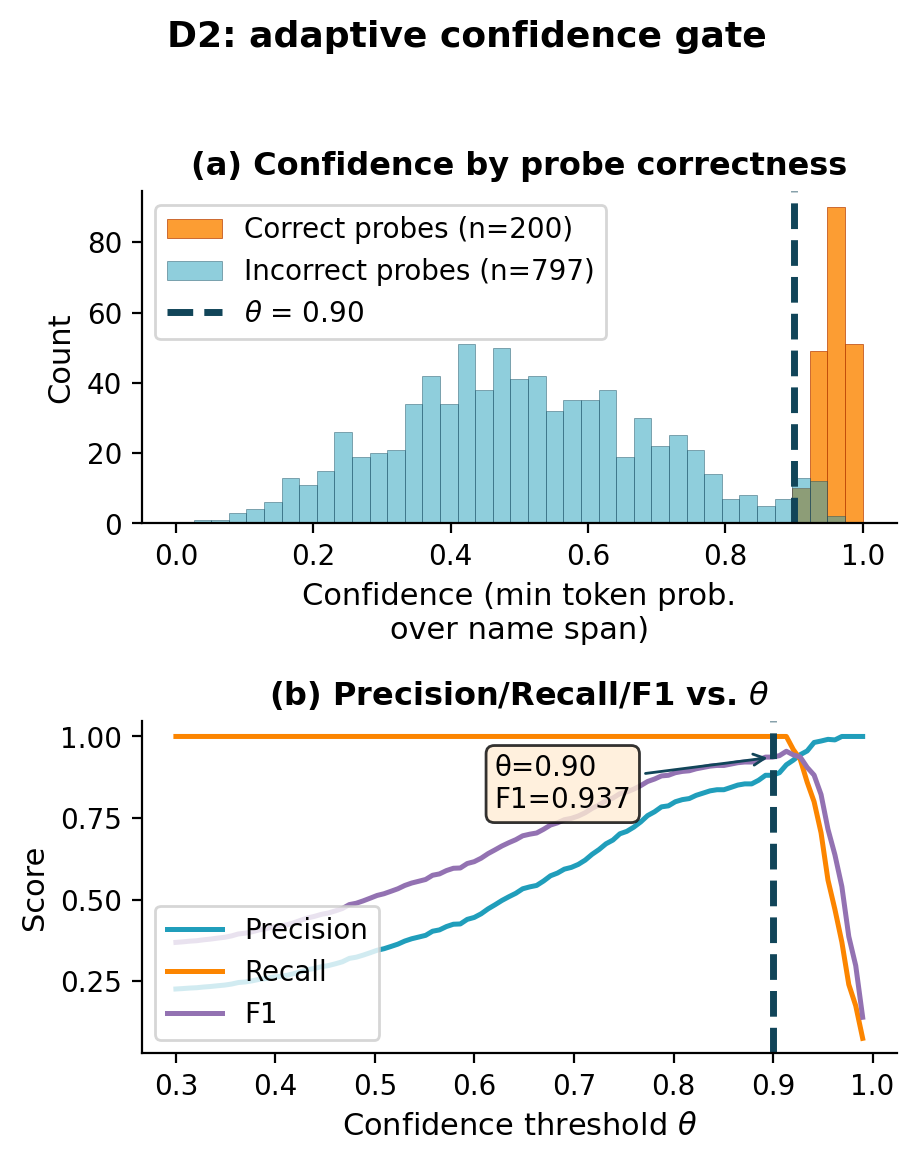
\includegraphics[width=0.86\columnwidth]{figures/fig_d2_confidence_gate.png}
  \caption{\textbf{D2 confidence gate threshold selection} (GAIA N=127, 997 probes).
  \textit{(a)}~Correct probes cluster above $\theta{=}0.90$; incorrect probes spread
  below. The threshold cleanly separates them.
  \textit{(b)}~Precision/Recall/F1 vs.\ $\theta$: the operating point $\theta{=}0.90$
  maximizes F1 (0.937) with 88\% precision and 100\% recall.
  D2 filters 77\% of probes (saving wasted tool executions) while committing every
  probe that would have been correct.}
  \label{fig:d2_gate}
\end{figure}

\subsection{D3: Partial-Token Accept for Rejected Probes}
\label{sec:d3}

When the strict gate rejects a probe, the main thread must otherwise generate the full tool
call from scratch (${\sim}50$ tokens, ${\sim}1.5$\,s at 32B scale).
Empirical analysis of 1268 probe--baseline pairs (BrowseComp,
Appendix~\ref{app:d3}) shows that even rejected probes match
the main's greedy output for the first $k$ tokens: mean $k \approx 29.5$, median 27,
$P_{25}=17$, $P_{75}=35$.

\parabf{Mechanism.}
D3 turns the probe into draft tokens for the main stream's \emph{own} speculative
decoding rather than re-decoding the tool call from scratch
(Figure~\ref{fig:d3_spec_dec}). We integrate a
\texttt{SporkProposer} into the serving engine's speculative-decoding proposer path:
as the main request decodes, the proposer watches for the \texttt{<tool\_call>}
boundary and, at that point, supplies the probe's tool-call body as the draft for
that request.
\begin{enumerate}
  \item When the main stream reaches the tool-call opener, the probe body is
        registered as the per-request draft.
  \item The engine verifies the draft against the main model in the same decode step
        (no separate verification pass, no second prompt); it accepts the longest
        prefix matching the main model's greedy tokens.
  \item The first $k$ matching tokens are accepted; the main stream decodes only the
        tool-call tokens after the first mismatch.
\end{enumerate}
D3 runs only in the in-process (engine) configuration, whose baseline is ngram
speculative decoding; the HTTP controller configuration (\S\ref{sec:implementation})
runs D1+D2 only.
D3 reduces the per-rejected-turn cost to approximately
$\Tbasestar + \Toh$, where $\Tbasestar = \Tbase - T_{\mathrm{D3}}$ is the realized base
decode after recycling the verified prefix as drafts ($\approx$0.6\,s per rejected turn,
$\approx$0.31\,s amortized per turn on BrowseComp; Appendix~\ref{app:d3}).
D3 is complementary to D1+D2: tool-level speculation on accepted turns, token-level
recycling on rejected turns; the fork itself is the draft, avoiding a separate draft model.

\begin{figure}[t]
  \centering
  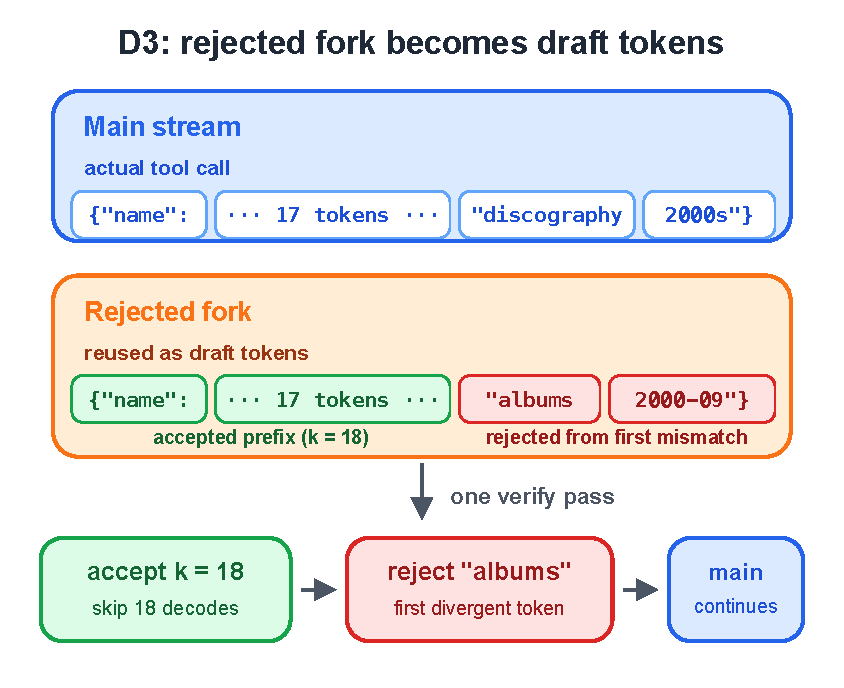
\includegraphics[width=0.95\columnwidth]{figures/fig_d3_spec_dec.pdf}
  \caption{\textbf{D3 treats the rejected fork as a draft for speculative verification.}
  Instead of discarding the probe, \spork{} verifies its tool-call tokens, accepts the
  longest matching prefix, and lets the main stream decode only the suffix after the first
  mismatch.}
  \label{fig:d3_spec_dec}
\end{figure}
